\documentclass[11pt,a4paper]{article}
\usepackage[margin=1in]{geometry}
\usepackage[T1]{fontenc}
\usepackage[utf8]{inputenc}
\usepackage{lmodern,microtype,amsmath,amssymb,graphicx,booktabs,array,longtable,tabularx}
\usepackage[authoryear,round]{natbib}
\usepackage[hidelinks]{hyperref}
\usepackage{placeins}
\setlength{\emergencystretch}{2em}
\renewcommand{\thetable}{S\arabic{table}}
\renewcommand{\thefigure}{S\arabic{figure}}
\graphicspath{{figures/}}
\title{Supplementary material\\Climate misinformation and quoted liquidity in energy equities}
\author{}\date{}
\begin{document}\maketitle
\section{Input provenance, sample, and reproducibility}
The financial input contains one row per security and calendar date. The content input contains one row per security and matched calendar date. Both keys are checked for uniqueness before a validated one-to-one merge. Model scores are fixed and are not reclassified, adjusted, or selected using financial outcomes. Exact input hashes, software versions, model formulas, coefficients, uncertainty estimates, sample sizes, and tail caps accompany the replication results.

The supplied financial panel has 204 securities and 198 distinct company names. Six company names have multiple securities: CNOOC, China Petroleum \& Chemical, China Shenhua Energy, PetroChina, Petrobras, and Shell. These include distinct listings and share classes; security identifiers are kept separate. Clustering by sector permits within-sector dependence among these securities. Company names are used only for the descriptive issuer count, not asserted to constitute a complete legal-entity identifier.

The index window ends on 13 October 2025, while the financial input continues to 31 December 2025. The 11,536 financial rows after the index endpoint, including 6,490 observed spreads, are not coded as unexposed observations in the estimation sample. Within the window, an absent matched post is coded as zero available matched content. This is a corpus convention, not a claim that no climate information circulated on that date.

The valid-score corpus has cross-sector disagreement in misinformation scores for 3.03\% of posts. For 1.19\%, the score crosses the threshold of 50 across sectors. The mean within-post score range is 1.161 points. Although the rubric requests industry-independent misinformation judgments, these observations show some context sensitivity. This diagnostic neither measures misclassification against ground truth nor supports a claim that the remaining agreement is accurate.

\begin{table}[htbp]
\centering
\caption{Estimation sample construction}
\label{tab:flow}
\begin{minipage}{\linewidth}
\small
\setlength{\tabcolsep}{4pt}
\begingroup\centering
\begin{tabular}{p{0.72\linewidth}r}
\toprule
Filter & Security-days \\
\midrule
Financial input & 726,890 \\
Within content window & 715,200 \\
Positive valid quotes and active trading & 489,929 \\
Contemporaneous-control complete cases & 486,655 \\
Prior-session-control complete cases & 485,800 \\
\bottomrule
\end{tabular}\par\endgroup
\par\vspace{0.5em}\footnotesize The two complete-case rows are alternative control choices applied to the same eligible quote sample, not sequential filters. Content window is 3 January 2012 to 13 October 2025. Active trading requires positive volume and a positive close.
\end{minipage}
\end{table}

\begin{table}[htbp]
\centering
\caption{Sector composition of the principal sample}
\label{tab:sectors}
\begin{minipage}{\linewidth}
\small
\setlength{\tabcolsep}{4pt}
\begingroup\centering
\begin{tabular}{p{0.50\linewidth}rrr}
\toprule
Energy sub-industry & Securities & Observations & Mean content \\
\midrule
Coal & 67 & 163,943 & 0.306 \\
Integrated Oil \& Gas & 11 & 35,317 & 0.540 \\
Oil \& Gas Drilling & 3 & 8,347 & 0.274 \\
Oil \& Gas Exploration and Production & 23 & 60,978 & 0.484 \\
Oil \& Gas Refining and Marketing & 28 & 78,441 & 0.402 \\
Oil \& Gas Transportation Services & 12 & 29,657 & 0.275 \\
Oil Related Services and Equipment & 15 & 28,137 & 0.260 \\
Renewable Energy Equipment \& Services & 40 & 76,259 & 0.348 \\
Renewable Fuels & 3 & 4,721 & 0.242 \\
\bottomrule
\end{tabular}\par\endgroup
\par\vspace{0.5em}\footnotesize Counts describe the principal estimation sample. Content is common within sector and date; observations are security-days.
\end{minipage}
\end{table}


\section{Listing-market crosswalk}
Exchange suffixes map to markets as follows: .SS and .SZ to mainland China; .HK to Hong Kong; .TW and .TWO to Taiwan; .T to Japan; .JK to Indonesia; .KL to Malaysia; .SA to Brazil; .L to the United Kingdom; .N, .OQ, and .O to the United States; .PA to France; .DE to Germany; and .AS to the Netherlands. The script fails if a security has an unmapped suffix. The complete crosswalk preserves the input region label for audit, but uses the exchange-based market for fixed effects.

Financial variables derived from a regional factor or regional macroeconomic mapping are not used as outcomes or controls in the principal analysis. A suffix-defined market-by-date effect does not require a regional risk-free rate, an assumed factor market, or a headquarters-country proxy. Security fixed effects and market-day effects also allow the financial controls to be used in local currency units without pooling their level differences as if they were comparable currency amounts. This does not resolve security-specific changes in shares outstanding or other source-data adjustments.

\section{Verified financial measurement identities}
Let $Q=(A+B)/2$ be the supplied midpoint and $V$ the supplied daily VWAP. For every nonmissing relevant observation, the following identities hold to numerical precision:
\begin{align}
\mathrm{SpreadPercent}&=100(A-B)/Q,\\
\mathrm{OrderFlow}&=V-Q,\\
\mathrm{PriceImpact}&=100\lvert V-Q\rvert/Q.
\end{align}
The latter two are source-column names. The signed gap has price units, rather than units of shares or signed traded value. The percentage gap has no trade-size denominator. They therefore do not identify order imbalance or a price-response coefficient. These identities are checked directly on 496,622 nonmissing gap observations and 504,043 spread observations in the financial input.

The reported quoted spread is likewise a daily quote summary. Its exact reconstruction establishes the formula but not the simultaneity of the component quotes, quote depth, or the effective spread of a particular transaction. Three crossed-quote observations and six nonpositive supplied spreads are present before sample selection. The estimation filter requires strictly positive bid and spread, ask at least bid, positive volume, and positive close. Daily range controls are explicitly computed from the supplied high, low, and close, rather than assigned a transaction-volatility interpretation.

\section{Classifier specification and measurement limits}
The saved model is Qwen3.6-35B-A3B-FP8. Its revision identifier is\\
\texttt{95a723d08a9490559dae23d0cff1d9466213d989}. The source run used vLLM 0.21 with temperature zero, FP8 weights, and a JSON grammar. Fixed decoding settings do not guarantee bitwise reproducibility across all hardware and inference implementations; the score files are the immutable input for the statistical replication.

The user prompt gives the energy sub-industry, the number of securities in its profile, countries and regions, and up to eight example companies. It then supplies the post date, content type, text truncated to 2,000 characters, link name and caption truncated to 200 characters each, and link description truncated to 400 characters. The truncation means that the classifier may not see all qualifying context. The system prompt asks for integer relevance and misinformation scores, a type label, and a rationale of at most 240 characters. Required JSON fields are \texttt{relevance}, \texttt{misinformation}, \texttt{misinfo\_type}, and \texttt{rationale}.

Relevance anchors distinguish unrelated content (0--10), general climate or energy content (11--30), broader energy-ecosystem relevance (31--60), clear sub-industry relevance (61--85), and directly sector-specific claims (86--100). Misinformation anchors distinguish no empirical claim or accurate content (0), minor spin (1--25), misleading framing or cherry-picking (26--50), clearly false or pseudoscientific claims (51--75), and egregious denial or fabrication (76--100). The prompt requests that misinformation be judged on the post's claims independently of industry, while relevance is sector-specific. Satire and quoted denial being refuted are assigned low scores, rather than automatically coded as false assertions.

The rubric-development inspection of 2,000 judgments identified problems in satire and unrelated political claims. Because those examples informed the rubric, they do not form a held-out validation set. The stored rationale is the classifier's explanation, not an independent human label or ground truth. The distributed input does not provide the original post text and link content needed for an independent annotation exercise. A score-based stratified validation-sample script is supplied to support such an exercise under authorized Meta access; it leaves human labels empty.

There are 217,998 distinct internal post identifiers among attempted outputs. Of these, 217,954 have at least one valid score. Failed outputs are not converted to zeros. Consequently, the attempted-judgment count is not exactly nine times the number of valid distinct posts. The post identifiers are internal integers and cannot be decoded into dates. The date map used to build the saved daily index is required to regenerate alternative post-subset daily measures.

\section{Why relevance thresholds change the estimand}
For threshold $c$, write $H_{pst}=1\{R_{ps}\geq c\}$. Three quantities must be kept distinct:
\begin{align}
 C^H_{st}(c)&=\frac{1}{n_{st}}\sum_p H_{pst}e_{ps},\\
 \bar e^H_{st}(c)&=\frac{\sum_p H_{pst}e_{ps}}{n^H_{st}(c)},\\
 q^H_{st}(c)&=n^H_{st}(c)/n_{st}.
\end{align}
When the high-relevance subset is nonempty, $C^H=q^H\bar e^H$. The composite mean decomposes as
\begin{equation}
 E_{st}=C^H_{st}(c)+C^L_{st}(c)
       =q^H_{st}(c)\bar e^H_{st}(c)+(1-q^H_{st}(c))\bar e^L_{st}(c).
\end{equation}
A regression on a conditional high-relevance mean can therefore have a different coefficient sign from a regression on $E$ even on the same dates. Its composition, denominator, and correlation with the subset share differ. This algebra makes a sign difference possible; it does not prove which component causes any observed difference. If $n^H=0$, the conditional mean is undefined. Replacing it by zero introduces an additional extensive-margin contrast, whereas the all-post contribution $C^H$ is legitimately zero.

The script \texttt{analysis/threshold\_aggregates.py} implements contributions and conditional means at thresholds 10, 25, 50, and 75 using the fixed scores and an authorized post-date crosswalk. It preserves missing conditional means for empty subsets and stops if scored post identifiers lack dates. The distributed replication inputs contain the daily composite and post-level scores but no post-date crosswalk. Therefore those thresholded daily regressors, and an irrelevant-post placebo reconstructed from them, are not treated as reproduced empirical checks in this paper. A null within-classifier placebo would in any event not establish classifier accuracy or causal specificity.

\section{Estimation and inference details}
All reported financial regressions use pyfixest 0.40.1. The underlying panel is sorted by security and date before forming session lags. An active session requires positive observed volume and a positive close. Lags are computed before quote and complete-case filtering, so a missing spread does not turn an older exposure into the previous day's value. A calendar-day lag instead joins date $t-1$ exactly. The latter excludes many Monday and holiday-adjacent observations because the financial panel is not a complete calendar-day series.

For the nested comparison, identical financial tail caps are applied to the same complete-case sample in all four specifications. In the principal model, outcome and prior-session controls are capped at their first and ninety-ninth sample percentiles, while the content variable is unchanged. Leave-out specifications preserve these principal-sample caps. Fixed-effect singleton observations are retained for transparent sample counts; a row with no within-effect variation contributes no identifying information.

Sector/date cluster covariance uses the two-way inclusion-exclusion estimator with package small-sample corrections and a $t_{8}$ reference for the nine-sector models. A leave-one-sector-out estimate has eight clusters and seven reference degrees of freedom. With so few clusters, both reference choices are approximations. The corresponding security/date covariance is an informative comparison, not the principal uncertainty measure.

Multiway inclusion-exclusion covariance matrices need not be positive semidefinite in finite samples. The analysis retains numerical warnings rather than silently changing the estimator. In the attention-adjusted model, the sector/date variance for the post-volume control is negative and its standard error is undefined. The reported composite-content standard error in that model remains finite. All principal-model coefficients and standard errors are finite, and no inference is drawn from an undefined control standard error. The machine-readable results preserve unavailable uncertainty measures as null values.

For date-score HAC, let $B=(\widetilde X'\widetilde X)^{-1}$ after absorbing all fixed effects, and let $a_t=\sum_{i\in t}(B\widetilde x_i)_j\hat u_i$ be the date-summed influence on coefficient $j$. The scalar covariance is
\begin{equation}
 \widehat V_L=\sum_t a_t^2+2\sum_{\ell=1}^{L}\left(1-\frac{\ell}{L+1}\right)
                              \sum_t a_ta_{t-\ell}.
\end{equation}
Dates are ordered observed dates, with bandwidths $L=5,20,60$. Reported HAC reference probabilities use the normal approximation. There is no additional finite-sample correction in this scalar diagnostic. It is not claimed to permit arbitrary dependence at all time horizons.

The sector sign calculation residualizes both exposure and outcome against nuisance controls and fixed effects under $\beta=0$. For sector $g$, let $s_g=\sum_{i\in g}\widetilde e_i\widetilde y_i$. The diagnostic compares $|\sum_gs_g|$ with the distribution of $|\sum_gw_gs_g|$ over all sign vectors $w_g\in\{-1,+1\}$. It is an unstudentized score sensitivity, rather than a finite-sample exact test: the independent symmetric-sector-score assumption is not guaranteed by the data. The analysis also verifies the exposure coefficient independently by the Frisch--Waugh--Lovell identity and reports each sector's share of residualized exposure variation.

\begin{table}[htbp]
\centering
\caption{Alternative inference for the principal coefficient}
\label{tab:inference}
\begin{minipage}{\linewidth}
\small
\setlength{\tabcolsep}{4pt}
\begingroup\centering
\begin{tabular}{p{0.57\linewidth}rr}
\toprule
Reference calculation & SE & $p$ \\
\midrule
Security/date clusters & 0.00108 & 0.188 \\
Sector/date clusters & 0.00220 & 0.533 \\
Date-score HAC, bandwidth 5 & 0.00225 & 0.524 \\
Date-score HAC, bandwidth 20 & 0.00223 & 0.521 \\
Date-score HAC, bandwidth 60 & 0.00201 & 0.476 \\
Sector score signs & --- & 0.512 \\
\bottomrule
\end{tabular}\par\endgroup
\par\vspace{0.5em}\footnotesize The coefficient and observations are identical in every row. Sector/date clustering has nine sectors. HAC uses ordered observed dates and a normal reference. Score signs enumerate 512 combinations and require independent symmetric sector scores; this is a diagnostic, not exact randomization inference.
\end{minipage}
\end{table}

\begin{table}[htbp]
\centering
\caption{Alternative content measures and attention adjustment}
\label{tab:variants}
\begin{minipage}{\linewidth}
\small
\setlength{\tabcolsep}{4pt}
\begin{tabular}{p{0.48\linewidth}rrr}
\toprule
Content regressor & Coefficient & SE & $p$ \\
\midrule
Mean composite & -0.0014 & 0.0022 & 0.533 \\
Log of one plus composite sum & 0.0002 & 0.0010 & 0.820 \\
Mean misinformation score & 0.0010 & 0.0013 & 0.470 \\
Mean relevance score & -0.0002 & 0.0004 & 0.644 \\
Share with misinformation at least 25 & 0.0338 & 0.0897 & 0.716 \\
Positive composite indicator & -0.0036 & 0.0040 & 0.398 \\
Composite with volume and relevance controls & -0.0013 & 0.0023 & 0.591 \\
\bottomrule
\end{tabular}
\par\vspace{0.5em}\footnotesize Principal controls and fixed effects throughout. Regressor units differ across rows; raw coefficient sizes are not comparable. The final row adds log one plus post count and mean relevance jointly. Sector/date inference.
\end{minipage}
\end{table}

\begin{table}[htbp]
\centering
\caption{Outcome, sample, and timing sensitivity}
\label{tab:sensitivity}
\begin{minipage}{\linewidth}
\footnotesize
\setlength{\tabcolsep}{4pt}
\begin{tabular}{p{0.40\linewidth}rrrr}
\toprule
Specification & Coefficient & SE & $p$ & N \\
\midrule
No financial controls & -0.0012 & 0.0017 & 0.492 & 485,800 \\
Unwinsorized spread and controls & -0.0086 & 0.0048 & 0.109 & 485,800 \\
Log spread & 0.0035 & 0.0020 & 0.122 & 485,800 \\
Matched-post dates only & -0.0014 & 0.0022 & 0.556 & 485,332 \\
Previous-session content & -0.0010 & 0.0022 & 0.652 & 485,759 \\
VWAP-midpoint percentage gap & 0.0010 & 0.0033 & 0.760 & 485,798 \\
\bottomrule
\end{tabular}
\par\vspace{0.5em}\footnotesize Unless stated otherwise the outcome is a percentage-point spread. Log spread and the VWAP gap have different units/interpretations. No gap outcome is interpreted as transaction price impact. Sector/date inference.
\end{minipage}
\end{table}

\begin{table}[htbp]
\centering
\caption{Leave-out diagnostics with fixed full-sample tail caps}
\label{tab:leaveout}
\begin{minipage}{\linewidth}
\footnotesize
\setlength{\tabcolsep}{4pt}
\begingroup\centering
\begin{tabular}{p{0.51\linewidth}rrr}
\toprule
Omitted sector or market & Coefficient & SE & $p$ \\
\midrule
Coal & -0.0013 & 0.0031 & 0.698 \\
Integrated Oil \& Gas & -0.0013 & 0.0026 & 0.635 \\
Oil \& Gas Drilling & -0.0020 & 0.0022 & 0.386 \\
Oil \& Gas Exploration and Production & -0.0010 & 0.0026 & 0.719 \\
Oil \& Gas Refining and Marketing & 0.0000 & 0.0027 & 0.992 \\
Oil \& Gas Transportation Services & -0.0015 & 0.0025 & 0.572 \\
Oil Related Services and Equipment & -0.0025 & 0.0021 & 0.266 \\
Renewable Energy Equipment \& Services & -0.0028 & 0.0025 & 0.296 \\
Renewable Fuels & -0.0006 & 0.0021 & 0.797 \\
Market: Mainland China & -0.0023 & 0.0032 & 0.482 \\
Market: Indonesia & 0.0002 & 0.0010 & 0.838 \\
Market: United States & -0.0020 & 0.0027 & 0.481 \\
\bottomrule
\end{tabular}\par\endgroup
\par\vspace{0.5em}\footnotesize All specifications retain the principal controls and fixed effects. Leaving out a sector leaves eight sector clusters. The full principal sample supplies tail caps; they are not recomputed within each leave-out sample.
\end{minipage}
\end{table}

\begin{table}[htbp]
\centering
\caption{Financial control definitions and tail caps}
\label{tab:controls}
\begin{minipage}{\linewidth}
\small
\setlength{\tabcolsep}{4pt}
\begingroup\centering
\begin{tabular}{p{0.55\linewidth}rr}
\toprule
Variable & Lower cap & Upper cap \\
\midrule
Quoted spread, percent & 0.0085 & 7.5381 \\
Prior log one plus volume & 7.9014 & 19.3589 \\
Prior log market capitalization & 20.1426 & 31.9419 \\
Prior range as percent of close & 0.0000 & 14.7036 \\
\bottomrule
\end{tabular}\par\endgroup
\par\vspace{0.5em}\footnotesize Principal sample first and ninety-ninth percentile caps. Exposure scores are not capped.
\end{minipage}
\end{table}

\FloatBarrier
\begin{figure}[htbp]\centering
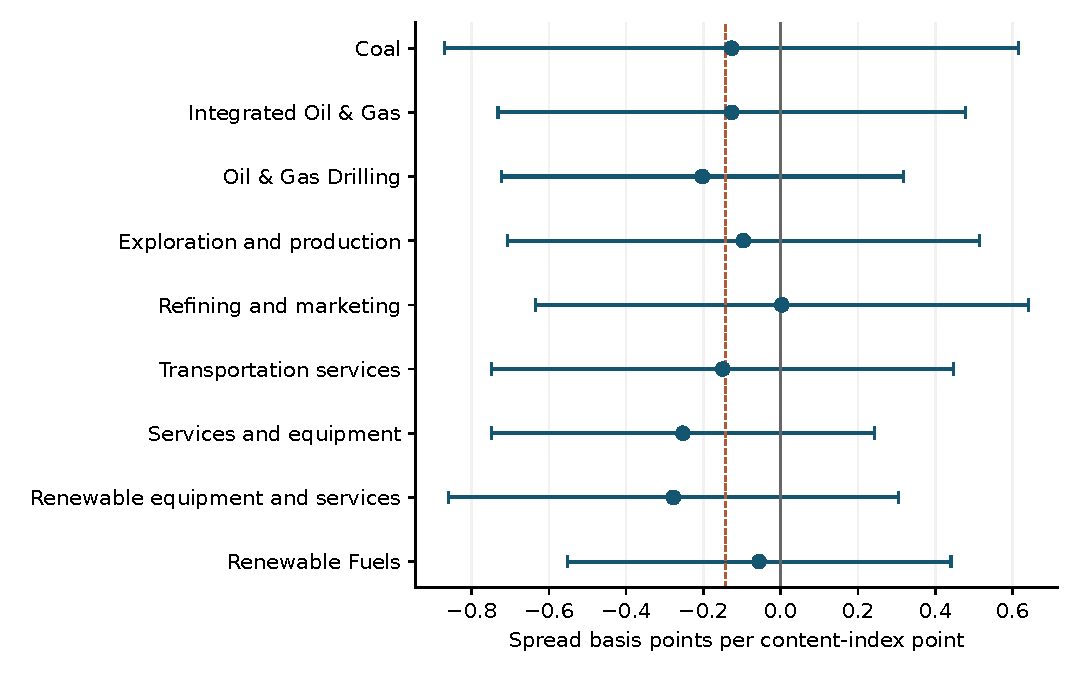
\includegraphics[width=\linewidth]{leave_sector_out.pdf}
\caption{Leave-one-sector-out coefficients using the principal model and fixed full-sample tail caps. Bars show approximate 95\% sector/date-clustered intervals with seven degrees of freedom. Source: reproducible Python computation from fixed inputs.}
\end{figure}
Across the nine sector leave-out fits, coefficients range from -0.0028 to 0.0000. These estimates assess concentration of the fitted association rather than supply nine independent confirmation tests. The matrix condition number of the principal within-transformed regressor matrix is 6.85. Its independently residualized coefficient equals -0.00143194, matching the fitted coefficient to numerical precision. A machine-readable results file records coefficients for every included control, the fixed-effect formula, tail caps, uncertainty estimates, and all model warnings.

\section{Scope of replication}
The distributed financial panel and daily score index are sufficient to regenerate every regression table and figure included here. The post-level shards are sufficient for product, error-count, and cross-sector consistency audits. Original text, the post-date crosswalk, audience geography, exchange-local posting timestamps, and transaction-level order direction are not supplied. No results based on those unavailable inputs are invented or silently reused. Independent human classification validation and causal identification remain outside the evidential scope of this analysis.
\end{document}
